\subsection{Off-Axis Fluxes}

The \nuprism detector concept exploits the fact that as a neutrino detector is moved to larger off-axis angles relative to the beam direction, the peak energy of the neutrino energy spectrum is lowered and the size of the high-energy tail is reduced. This effect can be seen in Figure~\ref{fig:offaxisfluxes}, which shows the neutrino energy spectra at several different off-axis angles in the T2K beam line.  Since the off-axis angle for a single neutrino interaction can be determined from the reconstructed vertex position, this extra dimension of incident neutrino energy dependence can be used to constrain the interaction rates and final state particles in a largely model independent way.

\begin{figure}[htpb]
    \begin{center}
      %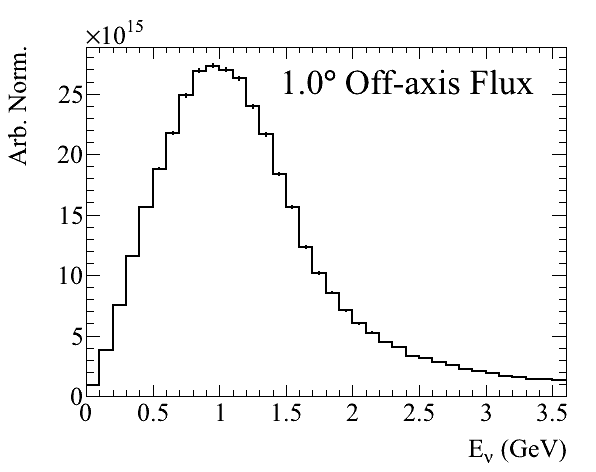
\includegraphics[width=\textwidth] {figures/oa_numu_flux_1deg.png}
      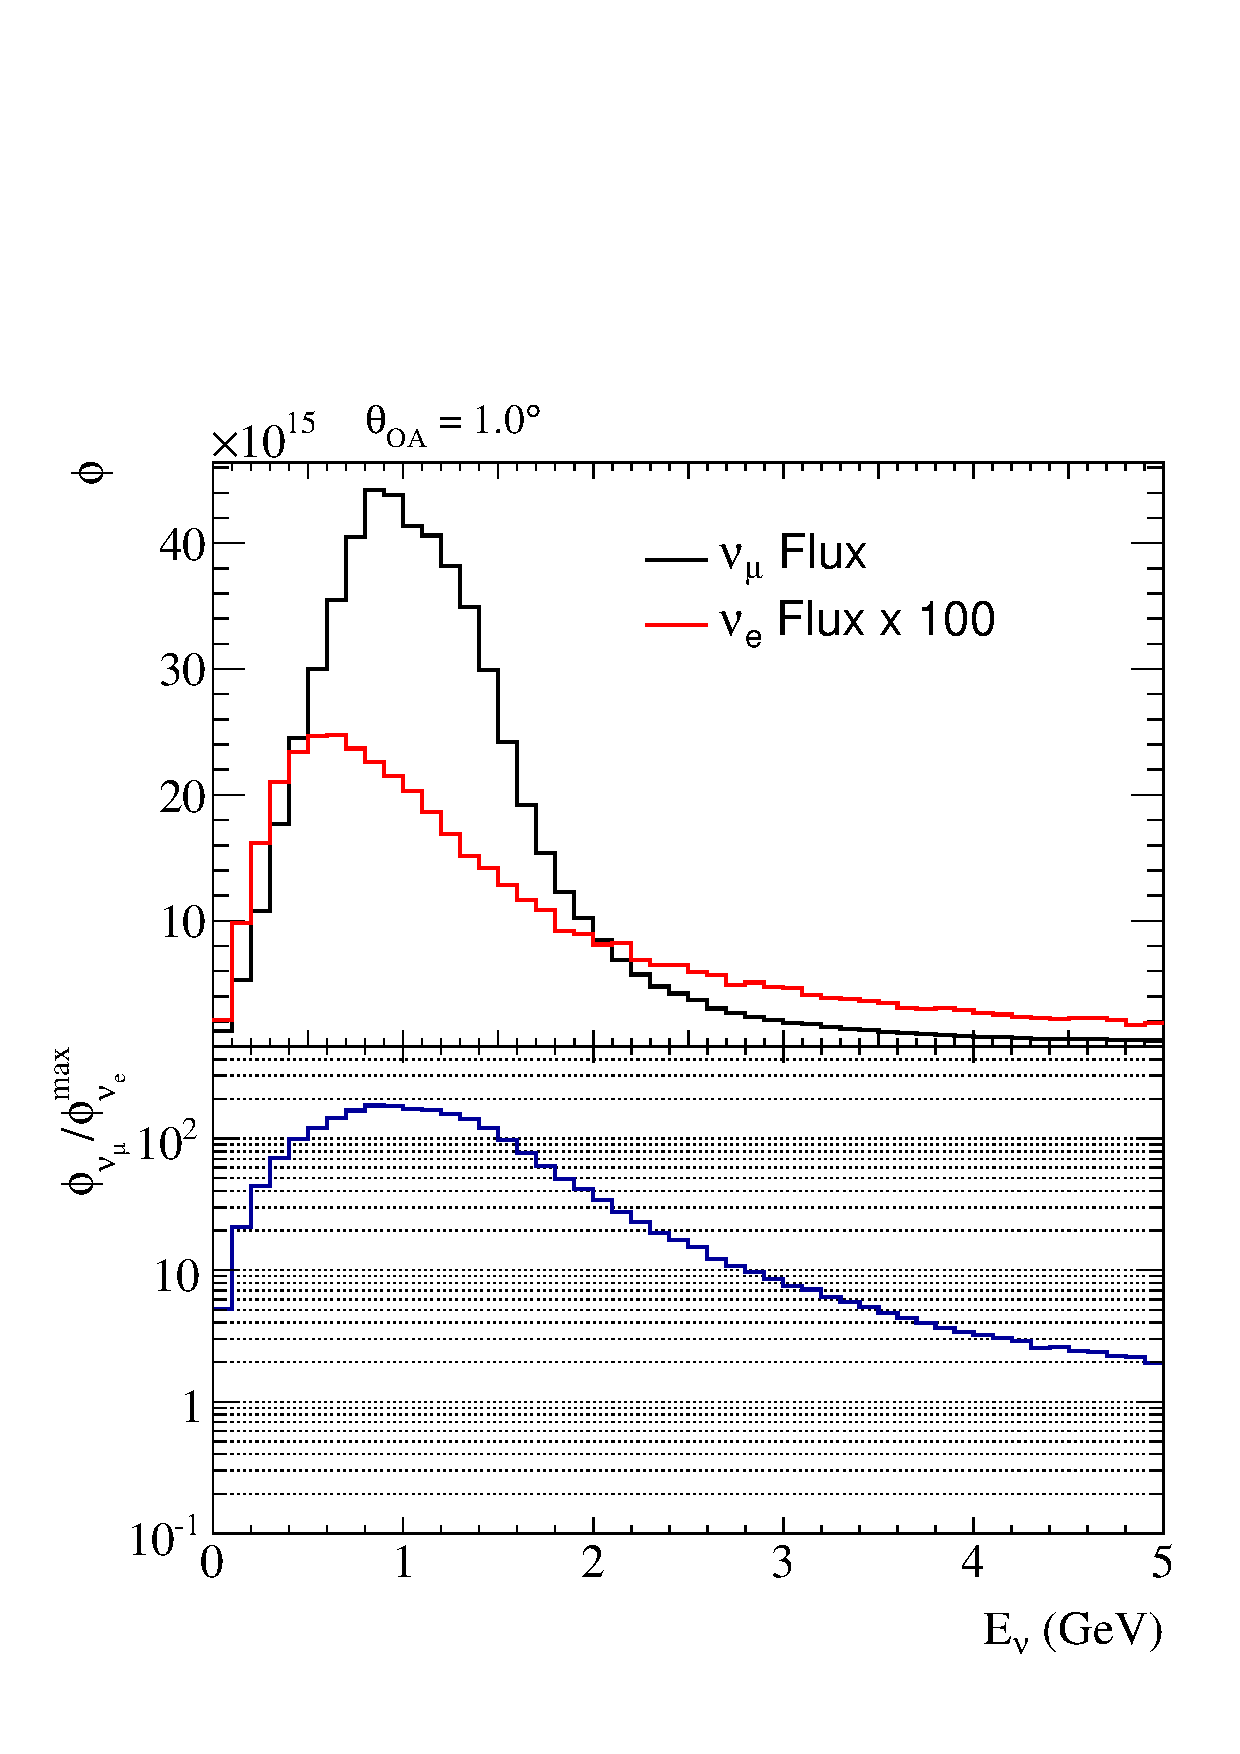
\includegraphics[width=6cm] {figures/nuprism_numu_nue_1p0deg.pdf}
      %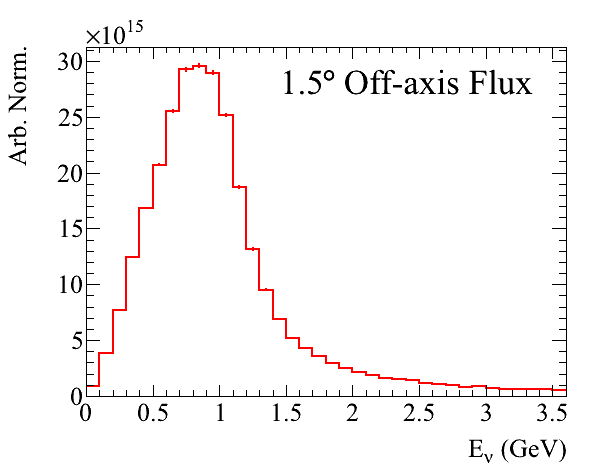
\includegraphics[width=\textwidth] {figures/oa_numu_flux_1p5deg.png}
%      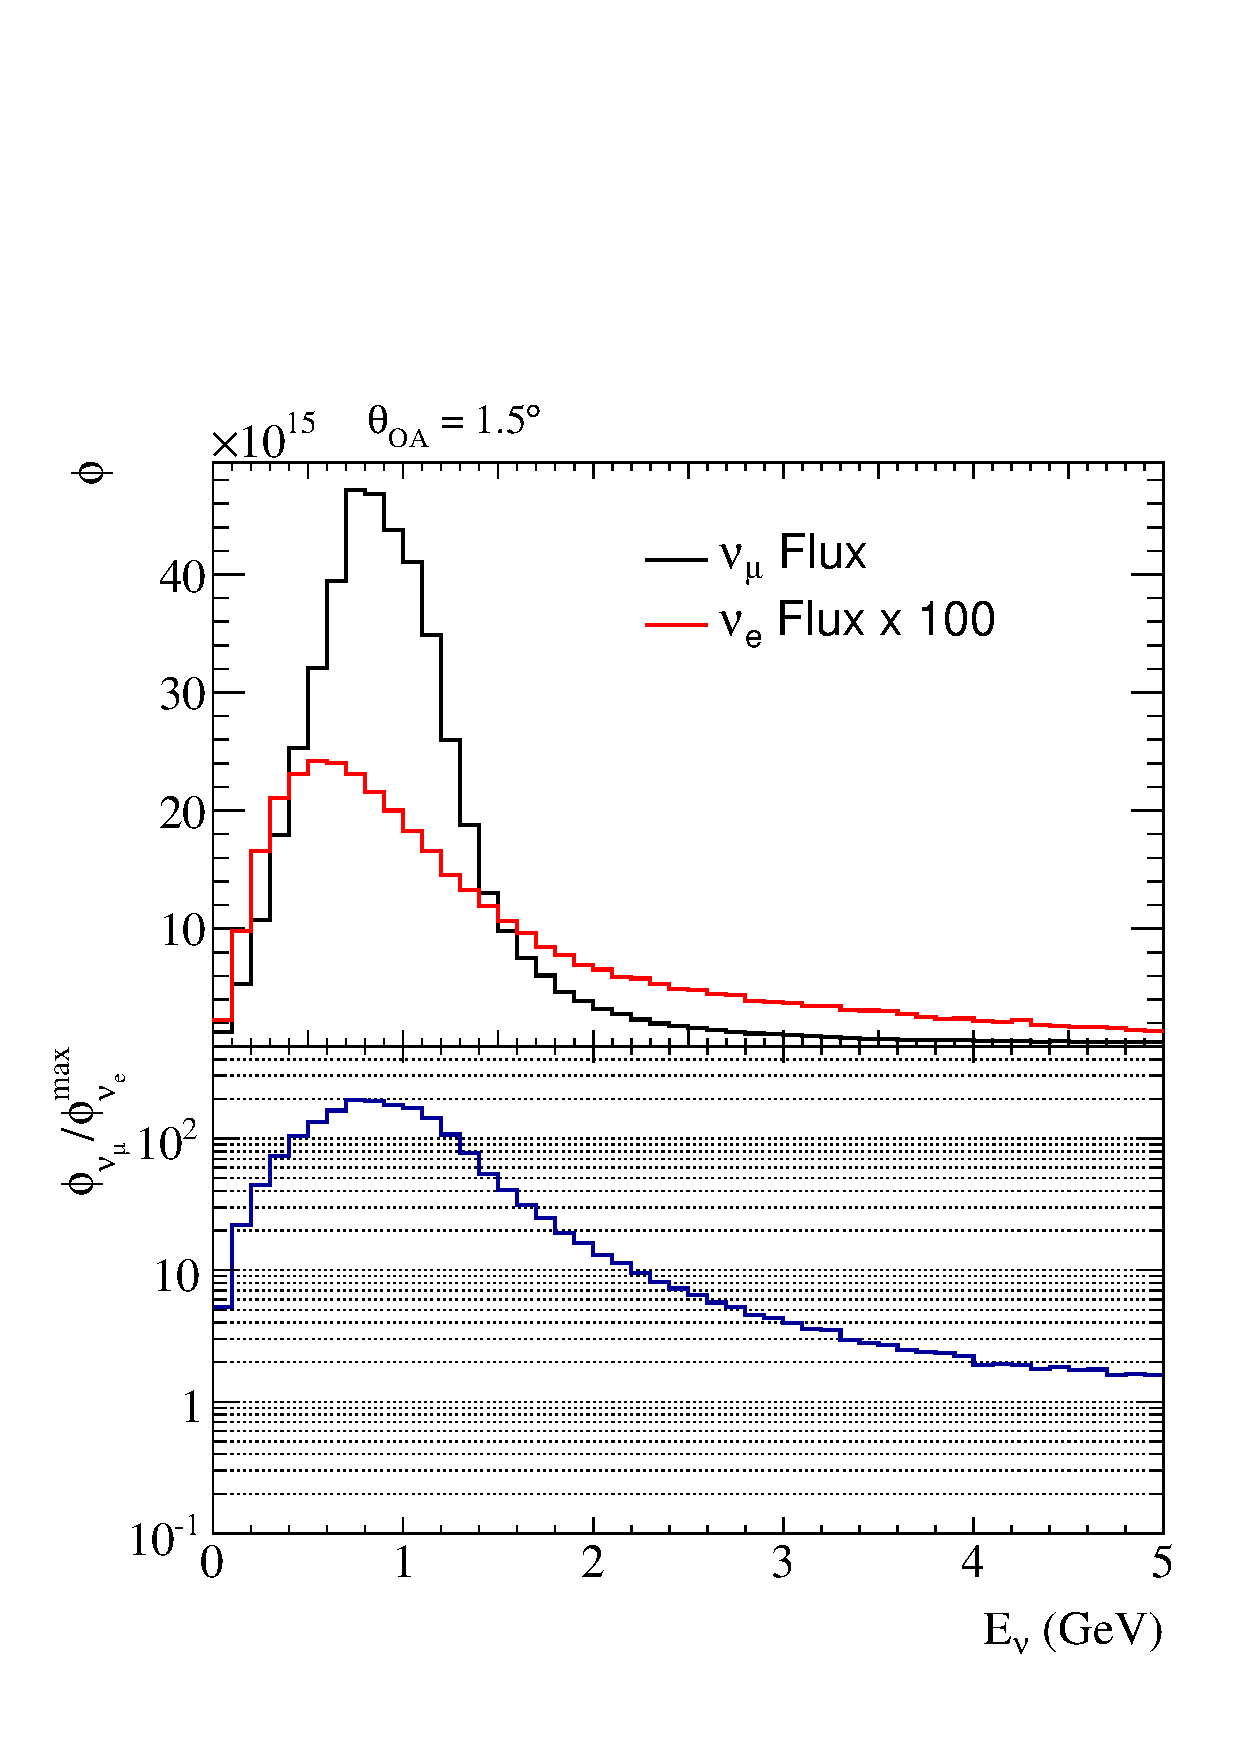
\includegraphics[width=4cm] {figures/nuprism_numu_nue_1p5deg.pdf}
      %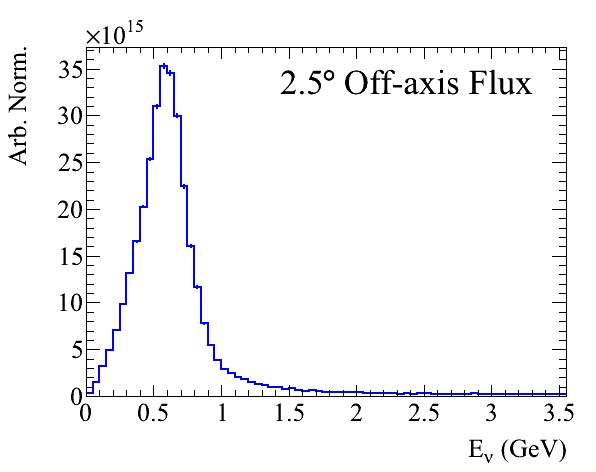
\includegraphics[width=\textwidth] {figures/oa_numu_flux_2p5deg.png}
      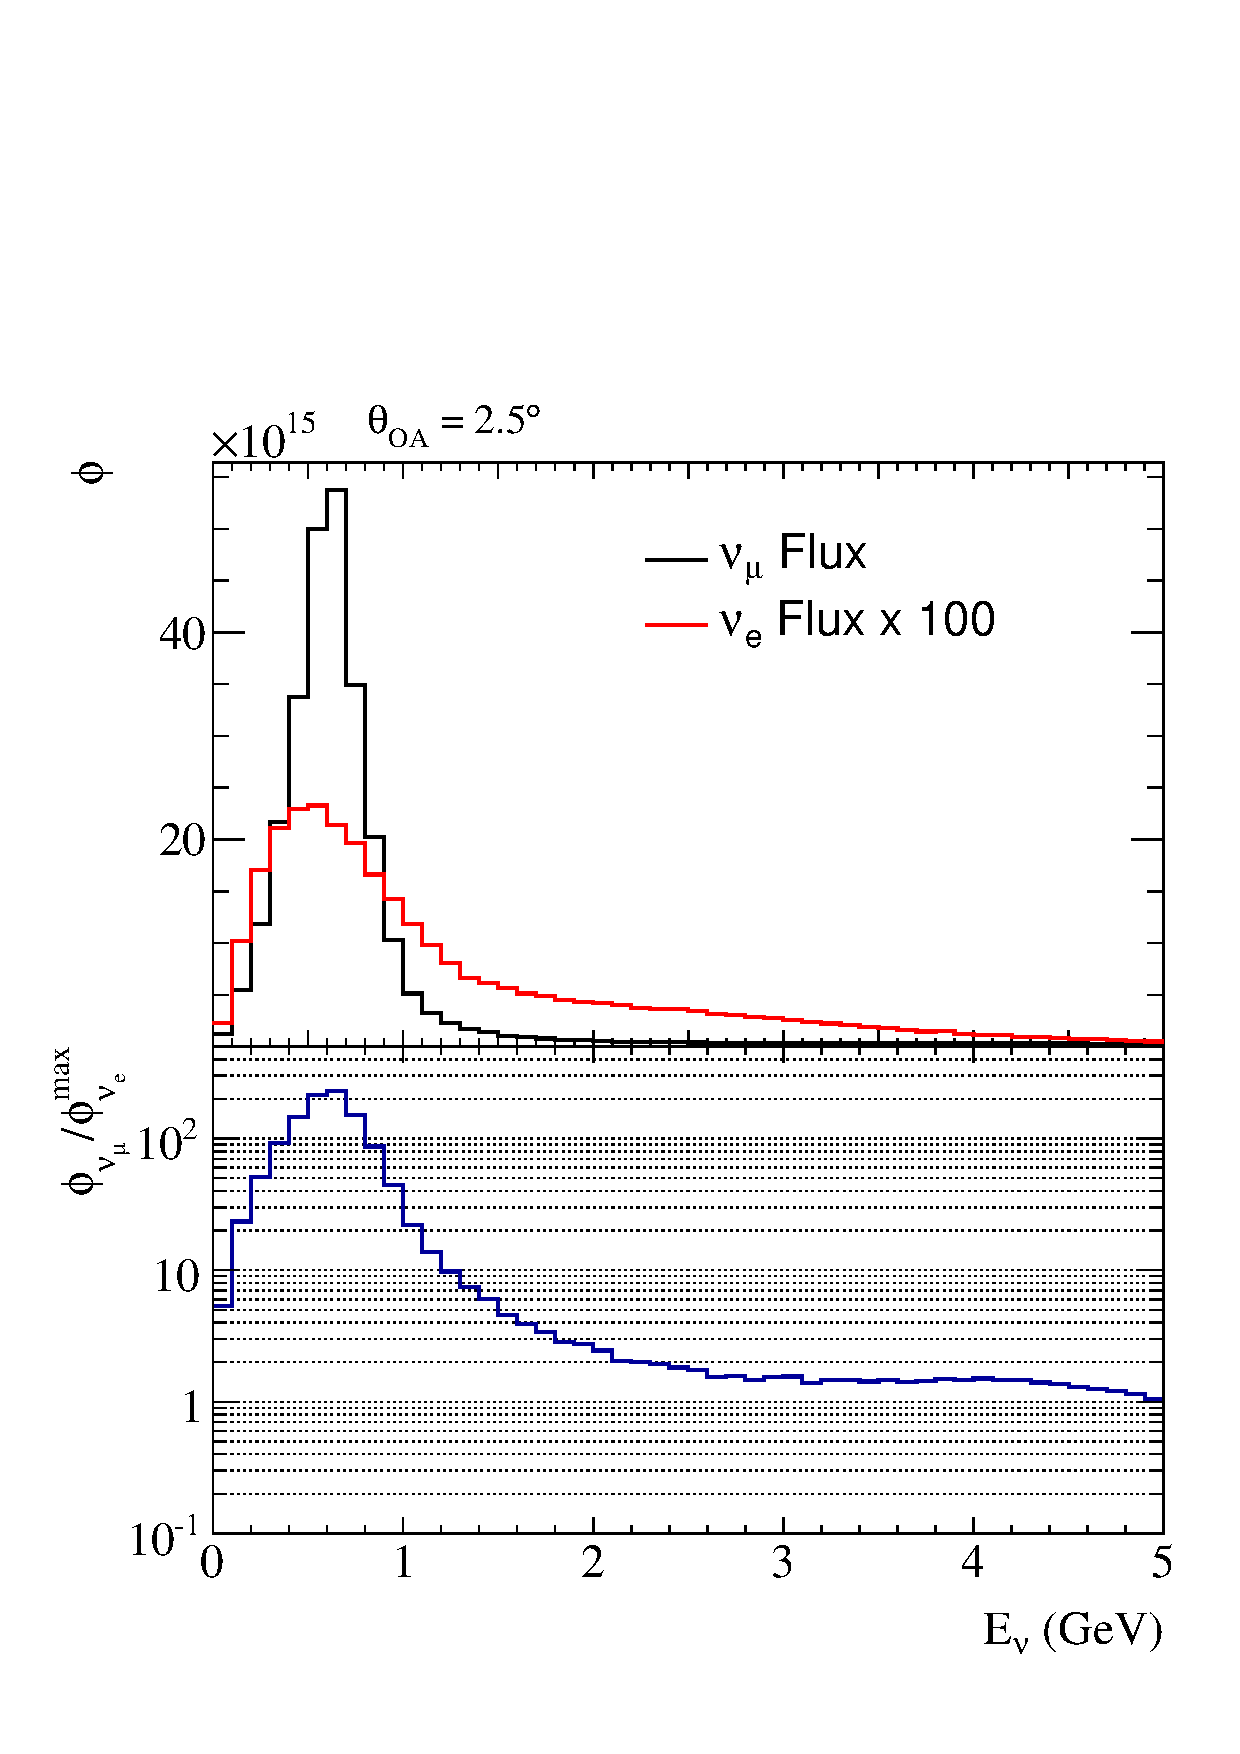
\includegraphics[width=6cm] {figures/nuprism_numu_nue_2p5deg.pdf}
      %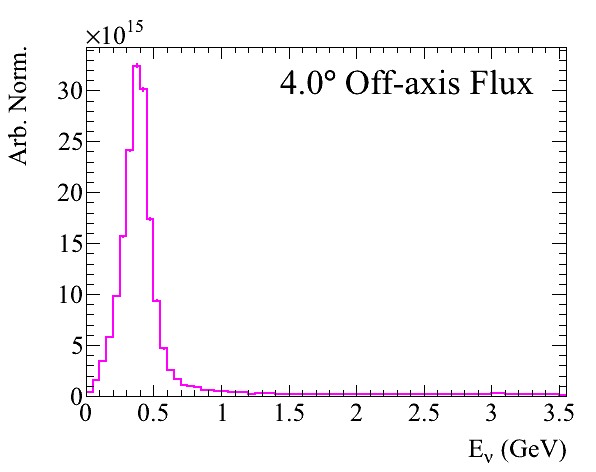
\includegraphics[width=\textwidth] {figures/oa_numu_flux_4deg.png}
      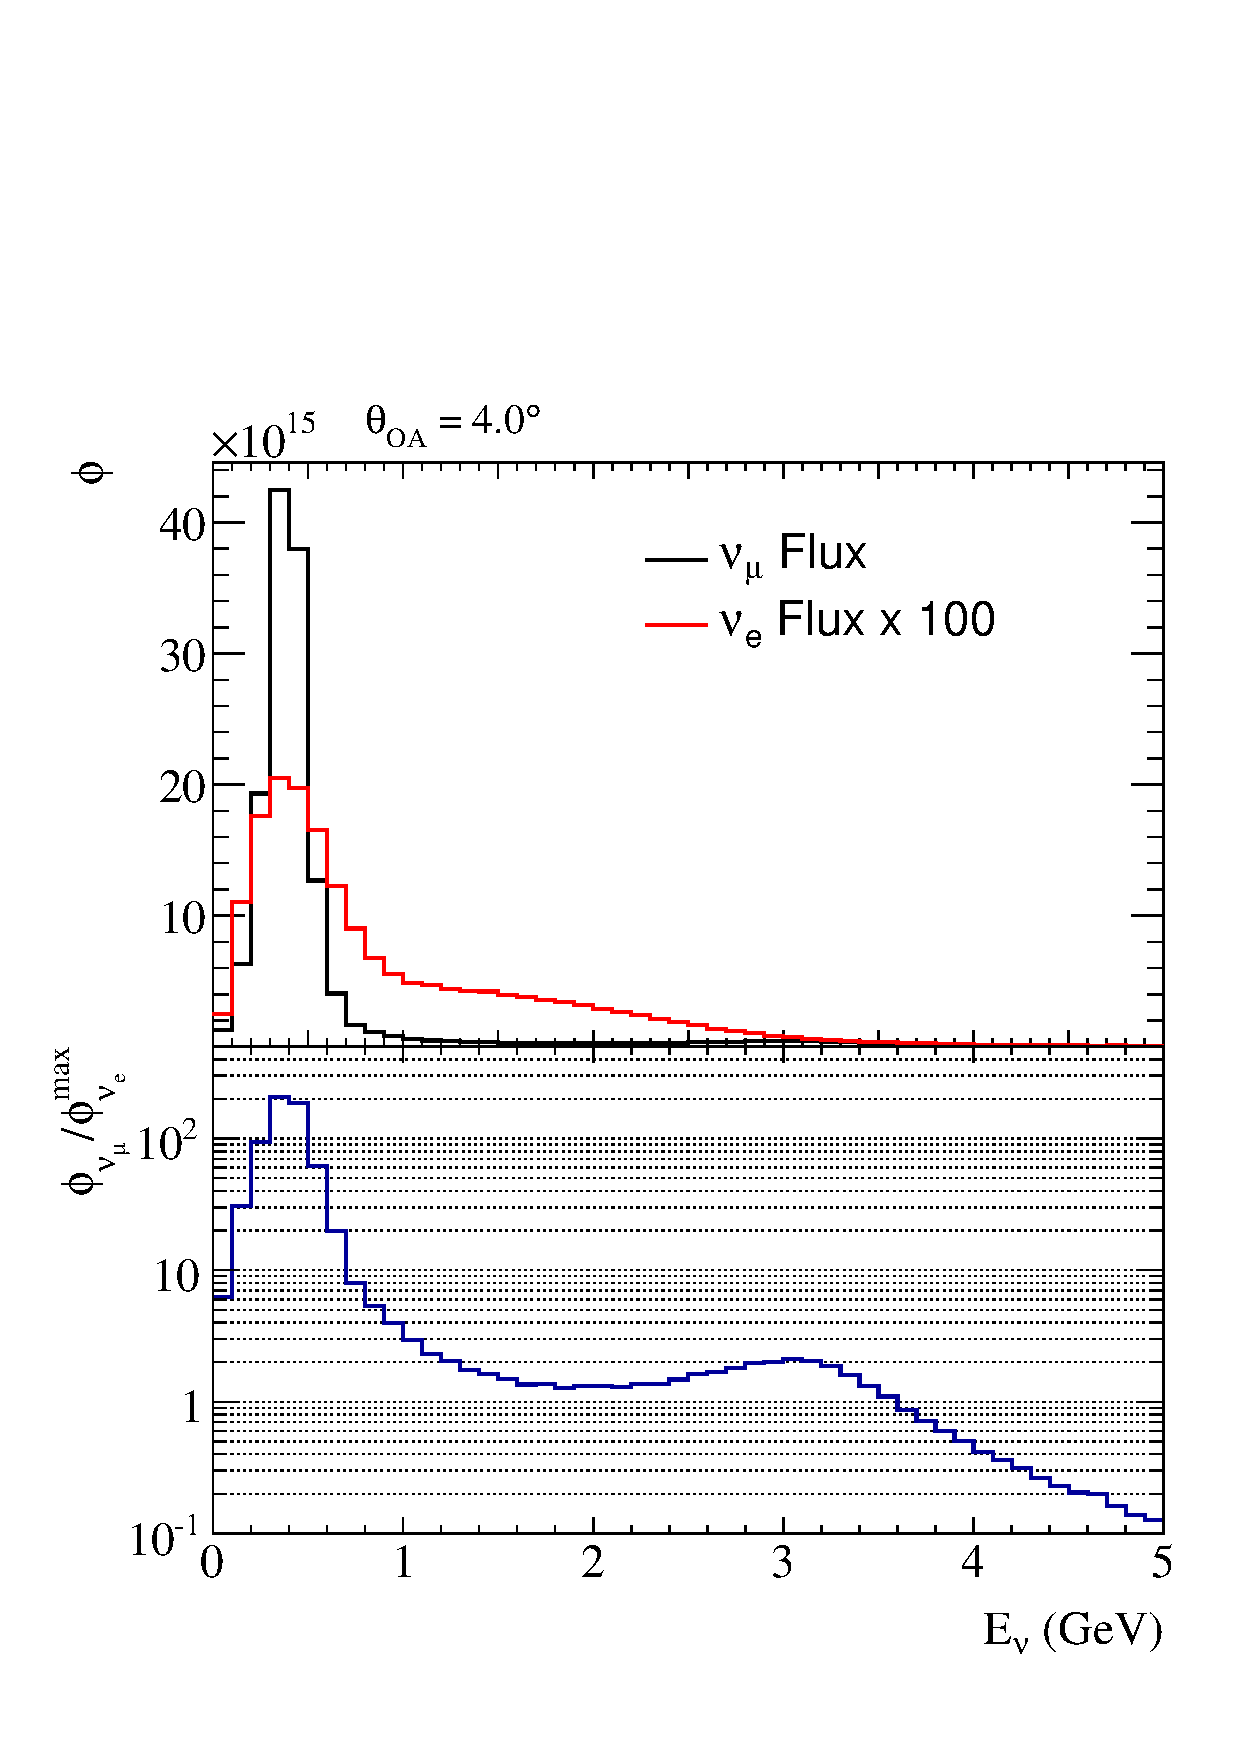
\includegraphics[width=6cm] {figures/nuprism_numu_nue_4p0deg.pdf}
    \end{center}
\caption{The neutrino energy spectra for $\nu_{\mu}$ and $\nu_{e}$ fluxes in the T2K beam operating in neutrino mode are shown for off-axis angles of 1$^{\circ}$, 2.5$^{\circ}$, and 4$^{\circ}$. The $\nu_{\mu}$ flux normalized by the maximum $\nu_e$ flux is shown at the bottom of each plot, demonstrating that feed-down from high energy NC backgrounds to $\nu_{e}$ candidates can be reduced by going further off-axis. }
\label{fig:offaxisfluxes}
\end{figure}

A typical \nuprism detector for the T2K beam line would span a continuous range of off-axis angles from 1$^\circ$ to 4$^\circ$. For T2K, the best choice of technology is a water Cherenkov detector in order to use the same nuclear target as Super-K, and to best reproduce the Super-K detector efficiencies.

\subsection{Monochromatic Beams}

The detector can be logically divided into slices of off-axis angle based on the reconstructed vertex of each
event. In each slice, the muon momentum and angle relative to the mean neutrino direction can be measured. By
taking linear combinations of the measurements in each slice, it is possible to produce an effective muon 
momentum and angle distribution for a Gaussian-like beam at energies between 0.4 and 1.2 GeV. Qualitatively, any
desired peak energy can be chosen by selecting the appropriate off-axis angle, as shown in Figure~\ref{fig:mono_beam}, and then
the further on-axis measurements are used to subtract the high energy tail, while the further off-axis 
measurements are used to subtract the low energy tail. Figure~\ref{fig:mono_beam} shows three such 
``pseudo-monochromatic" neutrino energy spectra constructed in this manner. These spectra are for selected 
1-ring muon candidates and systematic errors from the flux model are applied using the T2K flux systematic 
error model.  The statistical errors for an exposure of $4.5\times10^{20}$ protons on target are also shown. 
In all cases the high energy and low energy tails are mostly canceled over the full energy range and the 
monochromatic nature of the spectrum is stable under the flux systematic and statistical variations.

Figure~\ref{fig:mono_beam_erec} shows the reconstructed energy distributions for 1-ring muon candidates 
observed with the pseudo-monochromatic beams shown in Figure~\ref{fig:mono_beam}. The candidate events
are divided into quasi-elastic scatters and non-quasi-elastic scatters, which include contributions from
processes related to nuclear effects such as multinucleon interactions or pion absorption in final state
interactions.  With these pseudo-monochromatic beams, one sees a strong separation between the quasi-elastic 
scatters and the non-quasi-elastic scatters with significant energy reconstruction bias, especially in the
0.8 to 1.2 GeV neutrino energy range.  These measurements can be used to directly predict the effect of
non-quasi-elastic scatters in oscillation measurements and can also provide a unique constraint on nuclear 
models of these processes.

\begin{figure}[htpb]
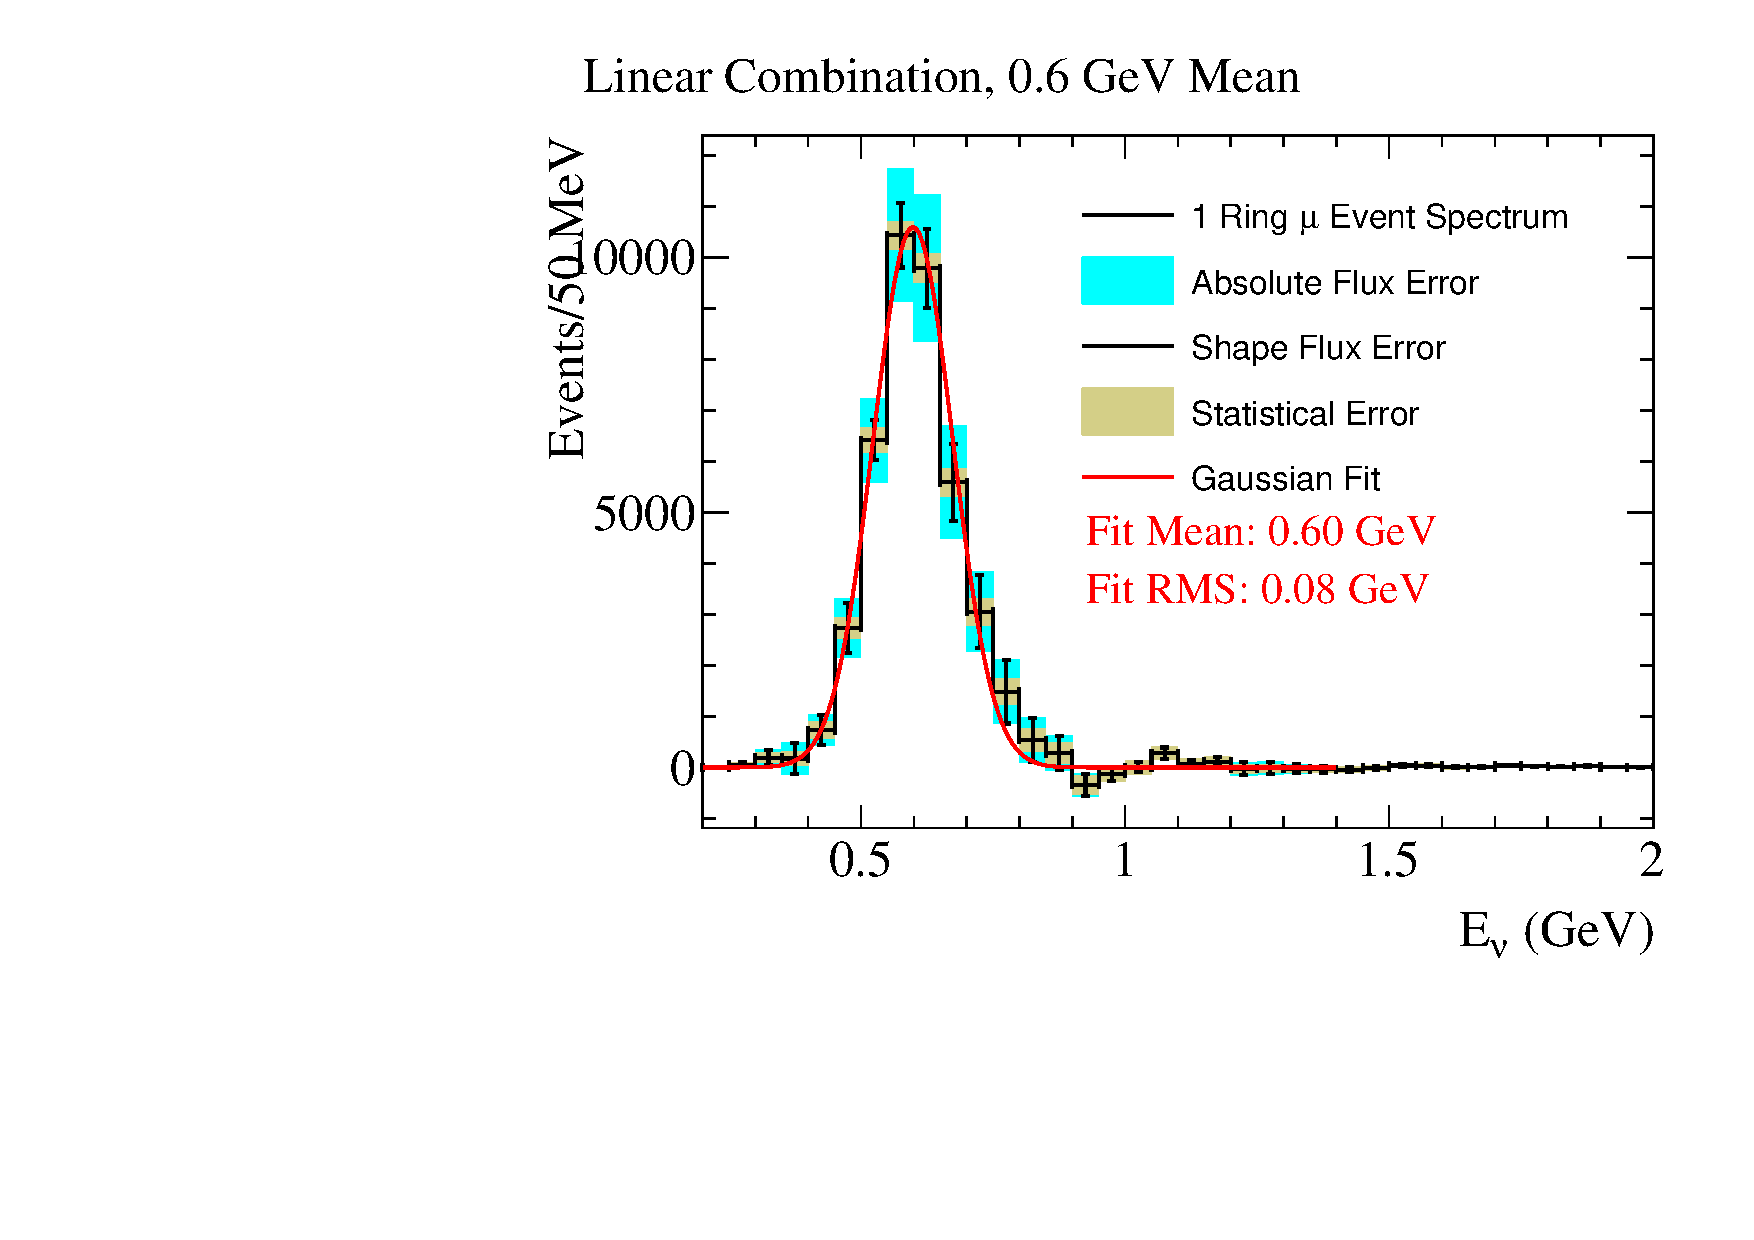
\includegraphics[width=0.45\textwidth]{figures/lc_etrue_600mev.pdf} \\
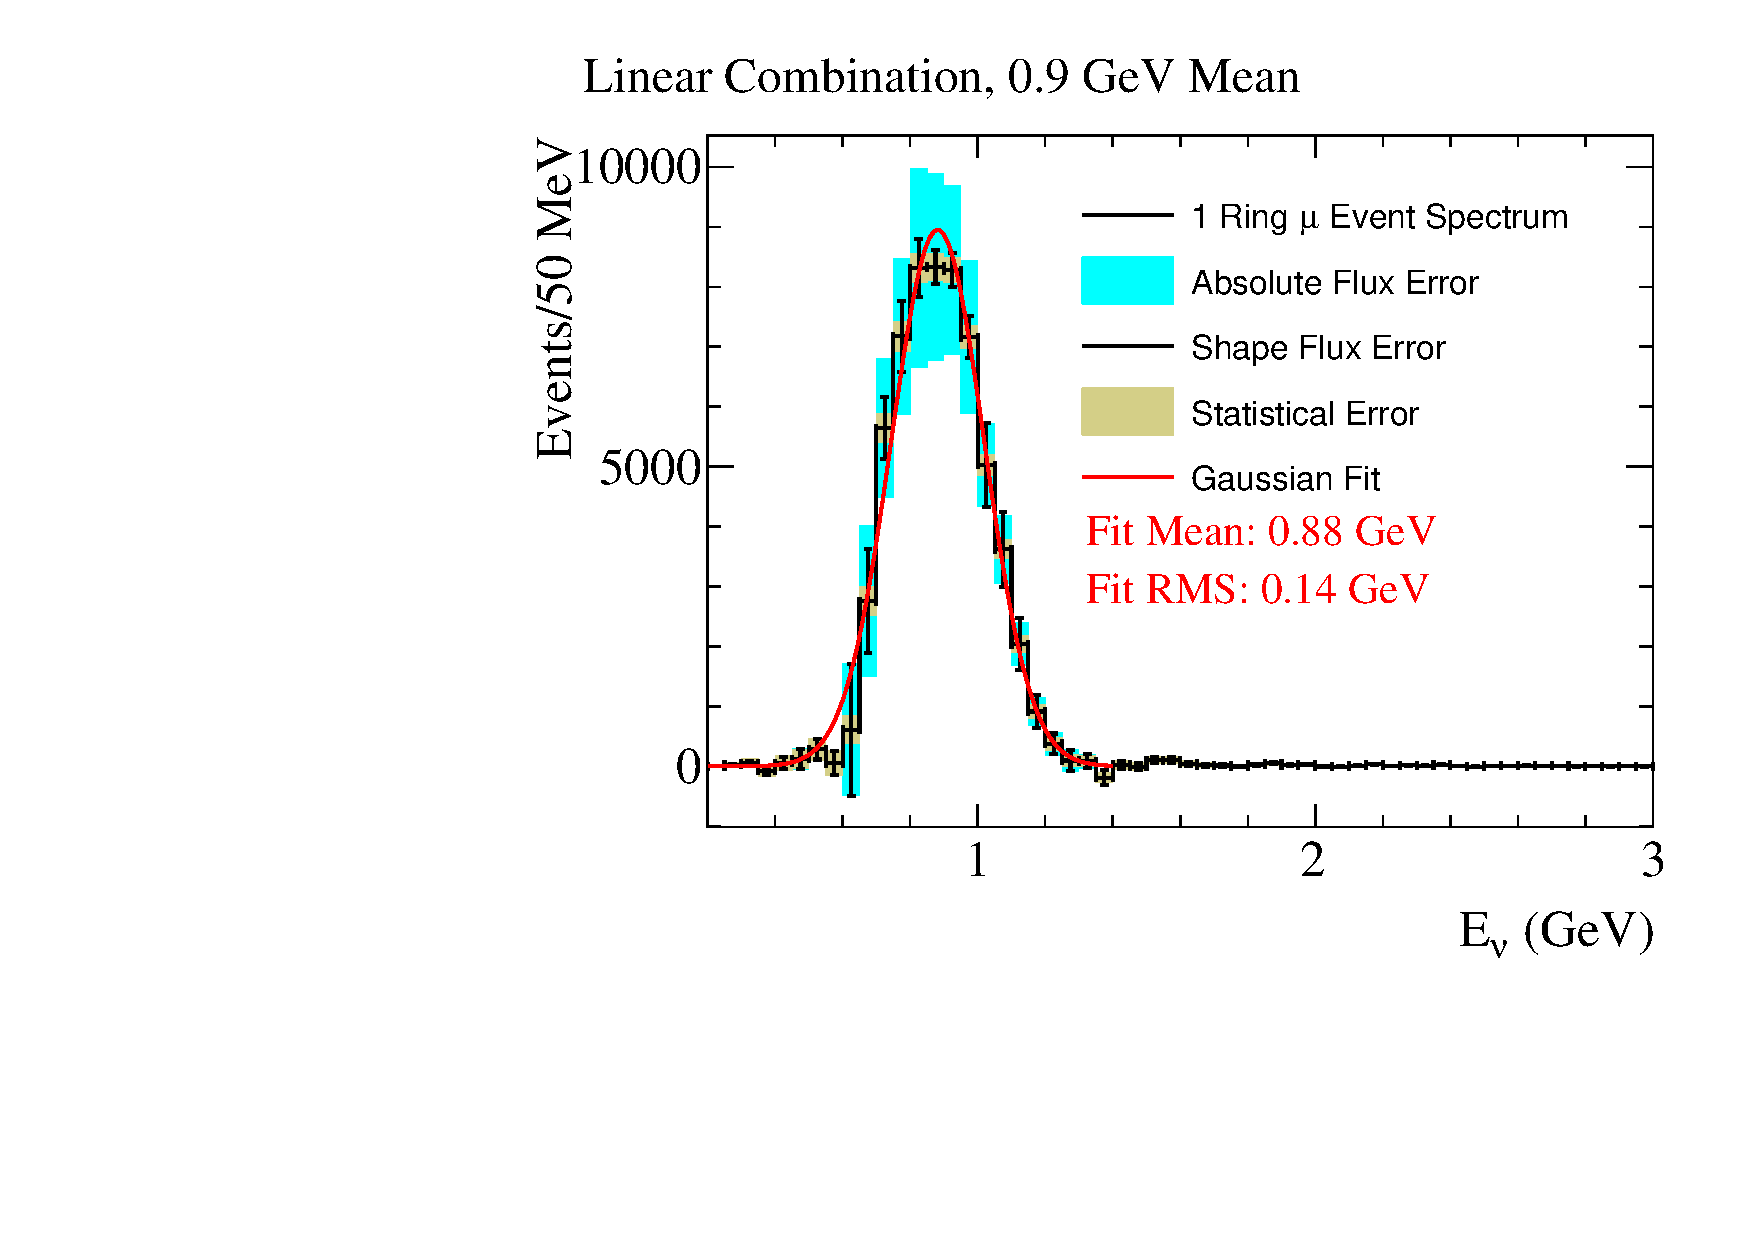
\includegraphics[width=0.45\textwidth]{figures/lc_etrue_900mev.pdf} \\
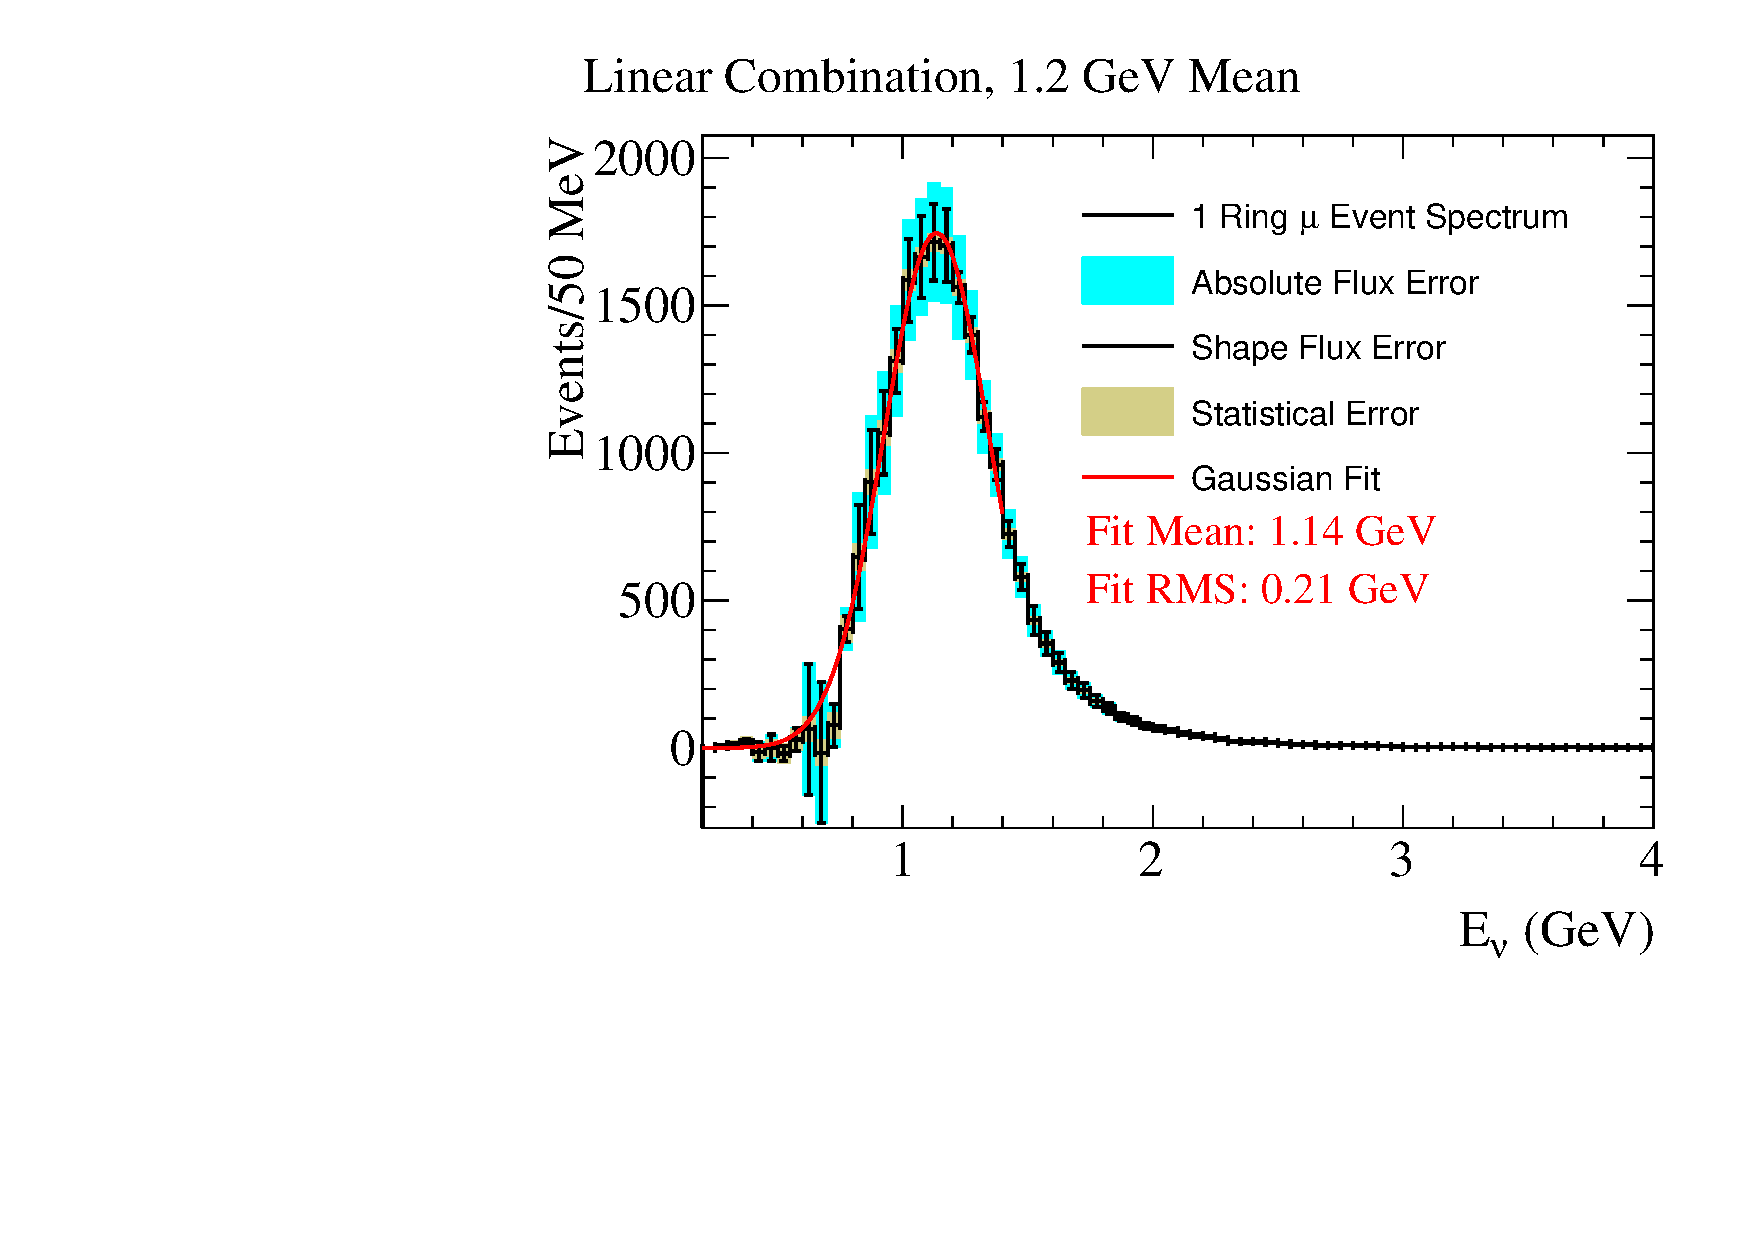
\includegraphics[width=0.45\textwidth]{figures/lc_etrue_1200mev.pdf} 
\caption{Three ``pseudo-monochromatic" spectra centered at 0.6 (top), 0.9 (middle) and 1.2 (bottom) GeV.  The aqua error bars show
the 1 $\sigma$ uncertainty for flux systematic variations, while the black error bars show the flux systematic variation after the
overall normalization uncertainty is removed.  The tan error bars show the statistical uncertainty for samples corresponding to 
 $4.5\times10^{20}$ protons on target.  }
\label{fig:mono_beam}
\end{figure}

\begin{figure}[htpb]
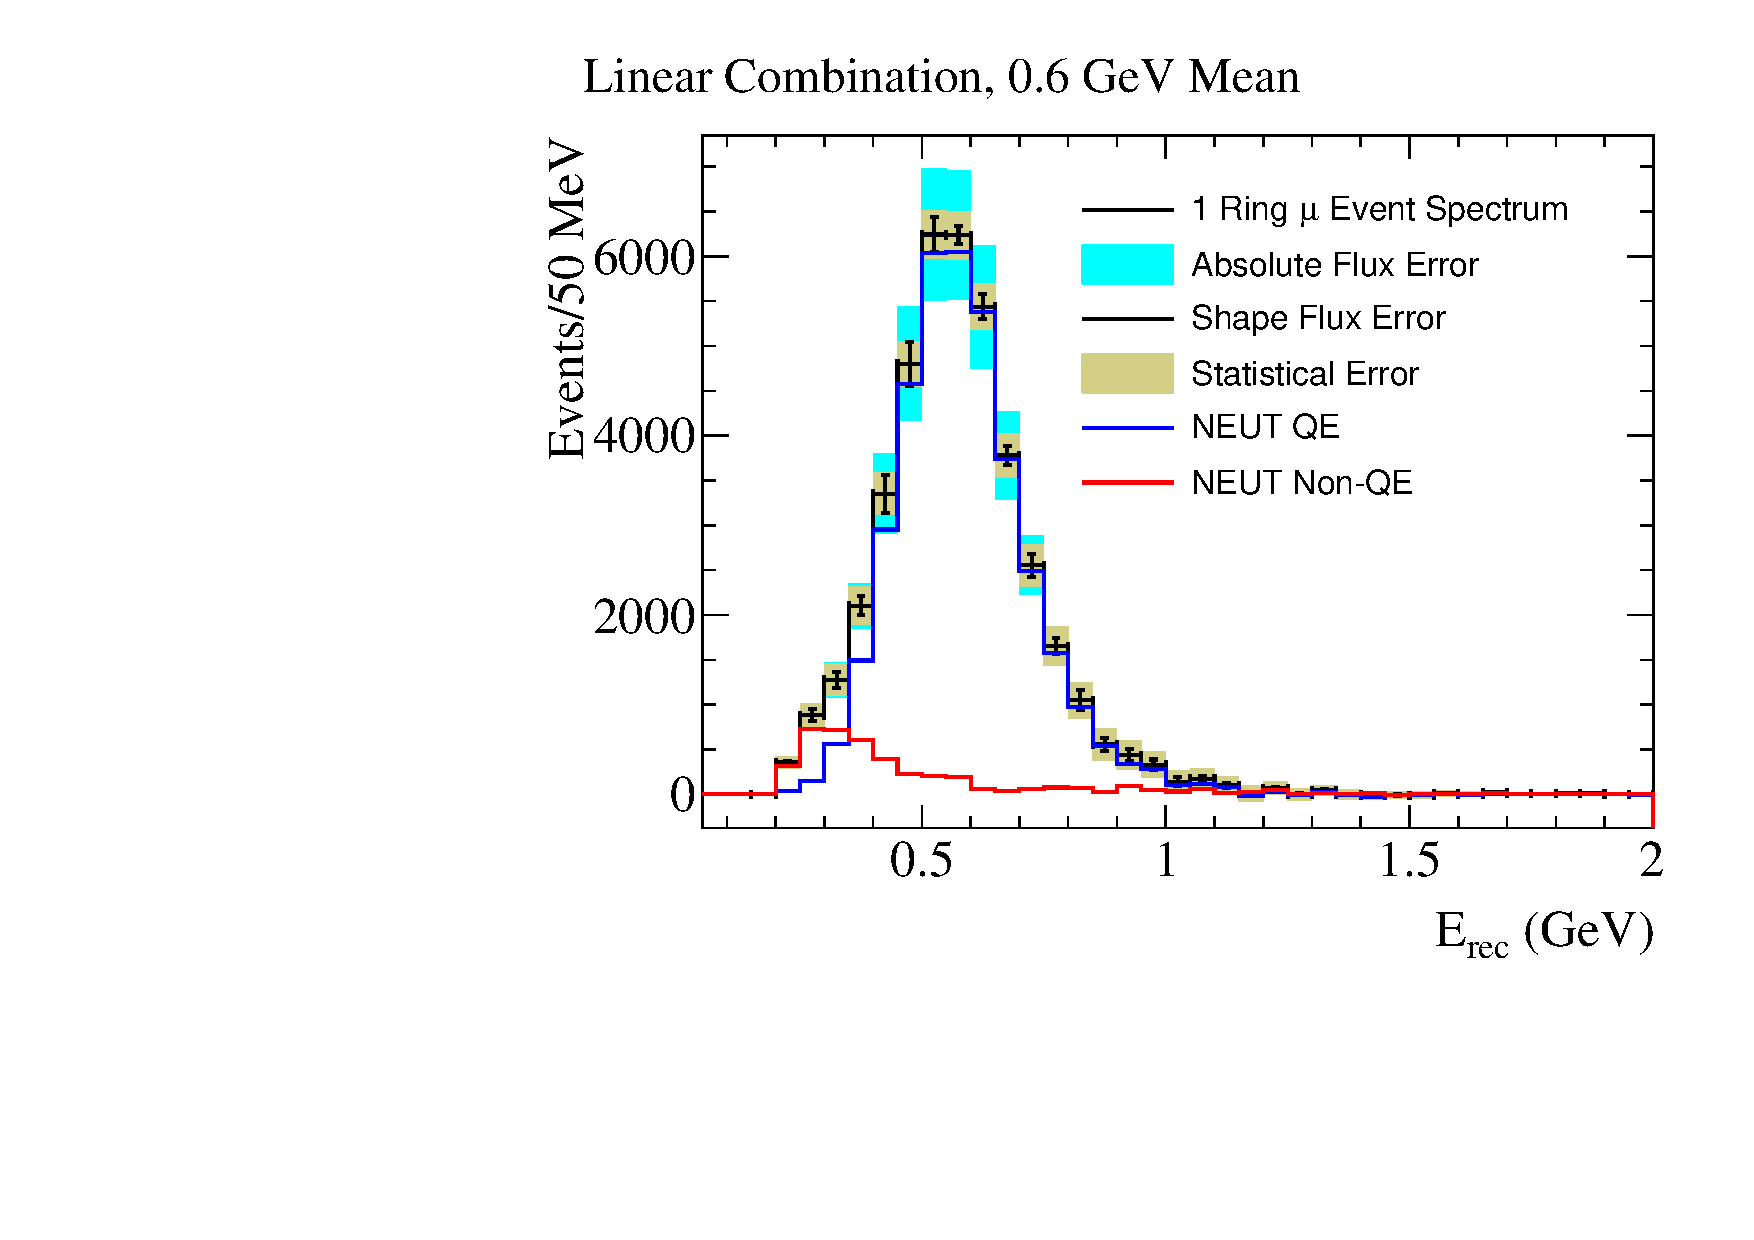
\includegraphics[width=0.45\textwidth]{figures/lc_erec_600mev.pdf} \\
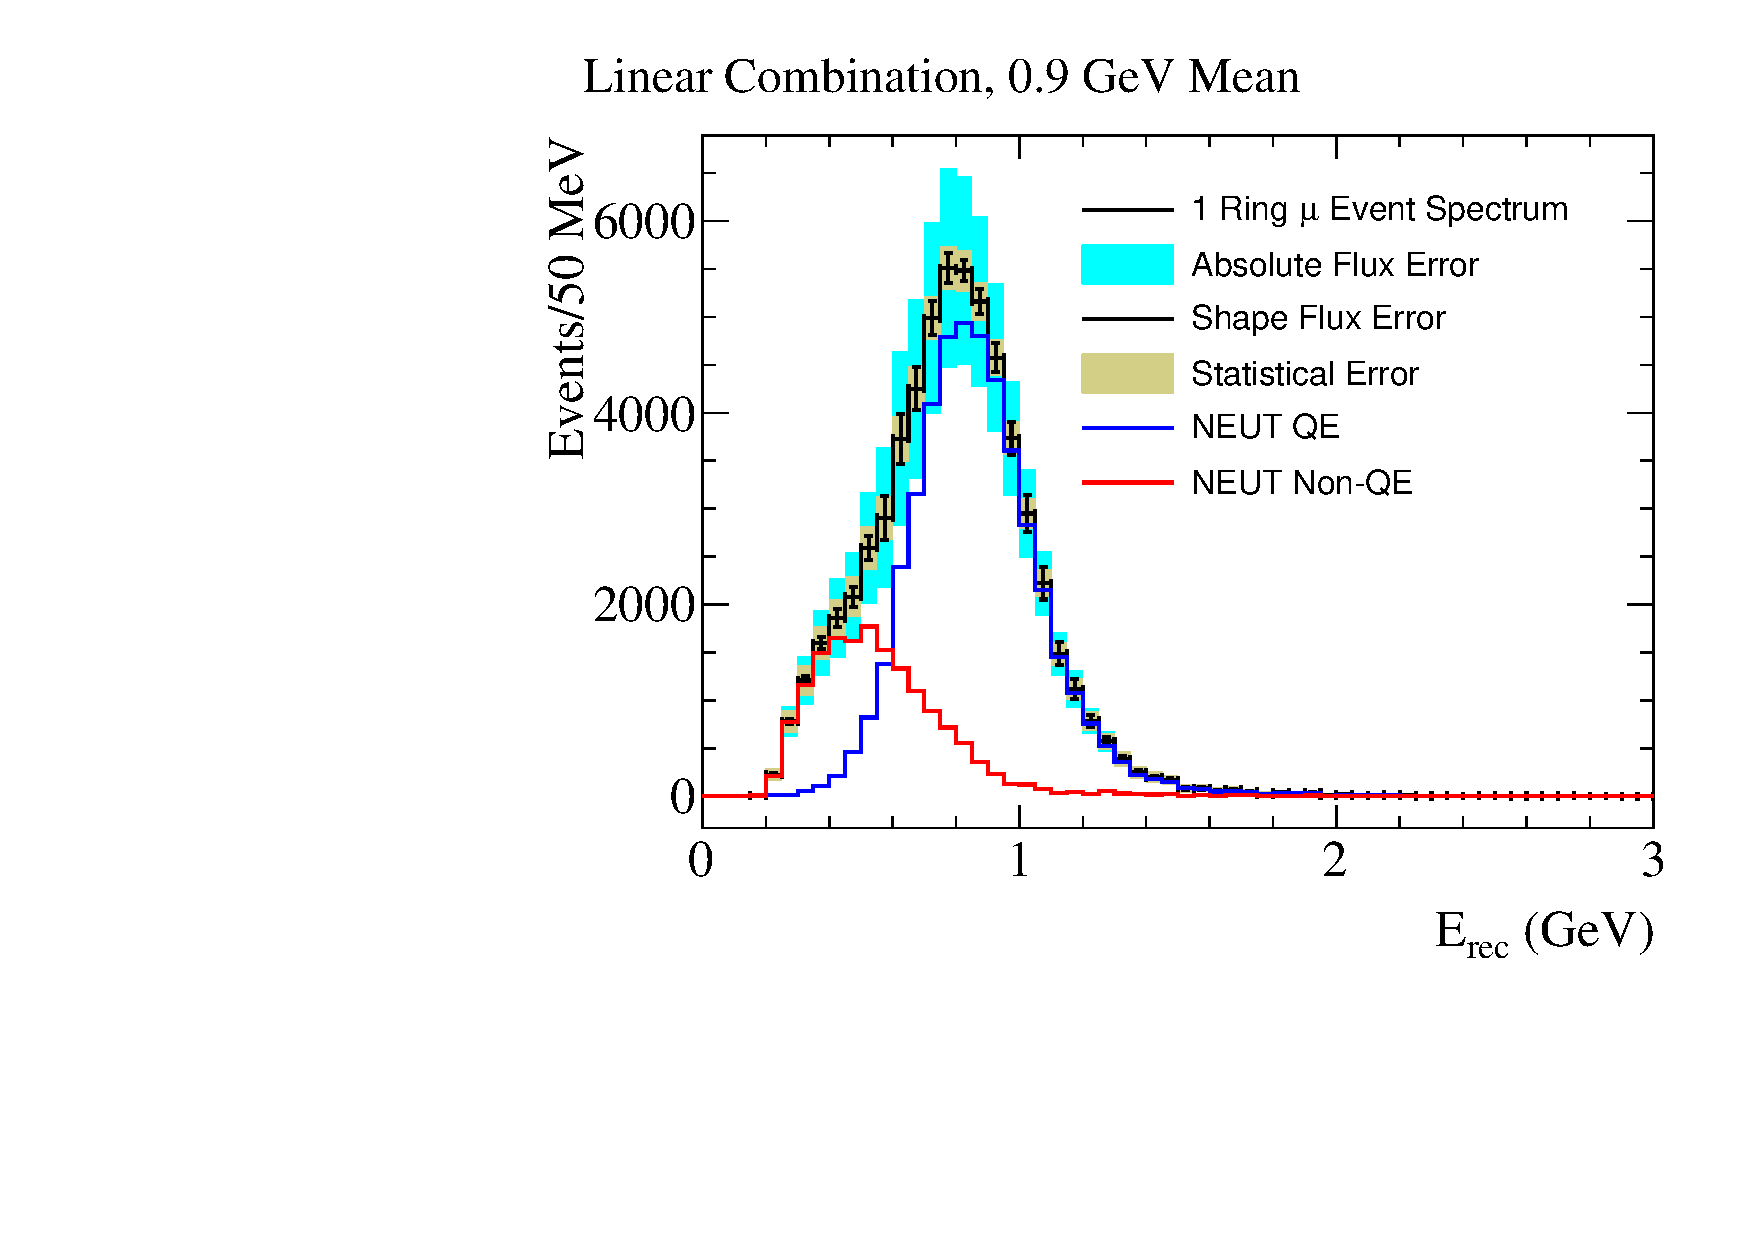
\includegraphics[width=0.45\textwidth]{figures/lc_erec_900mev.pdf} \\
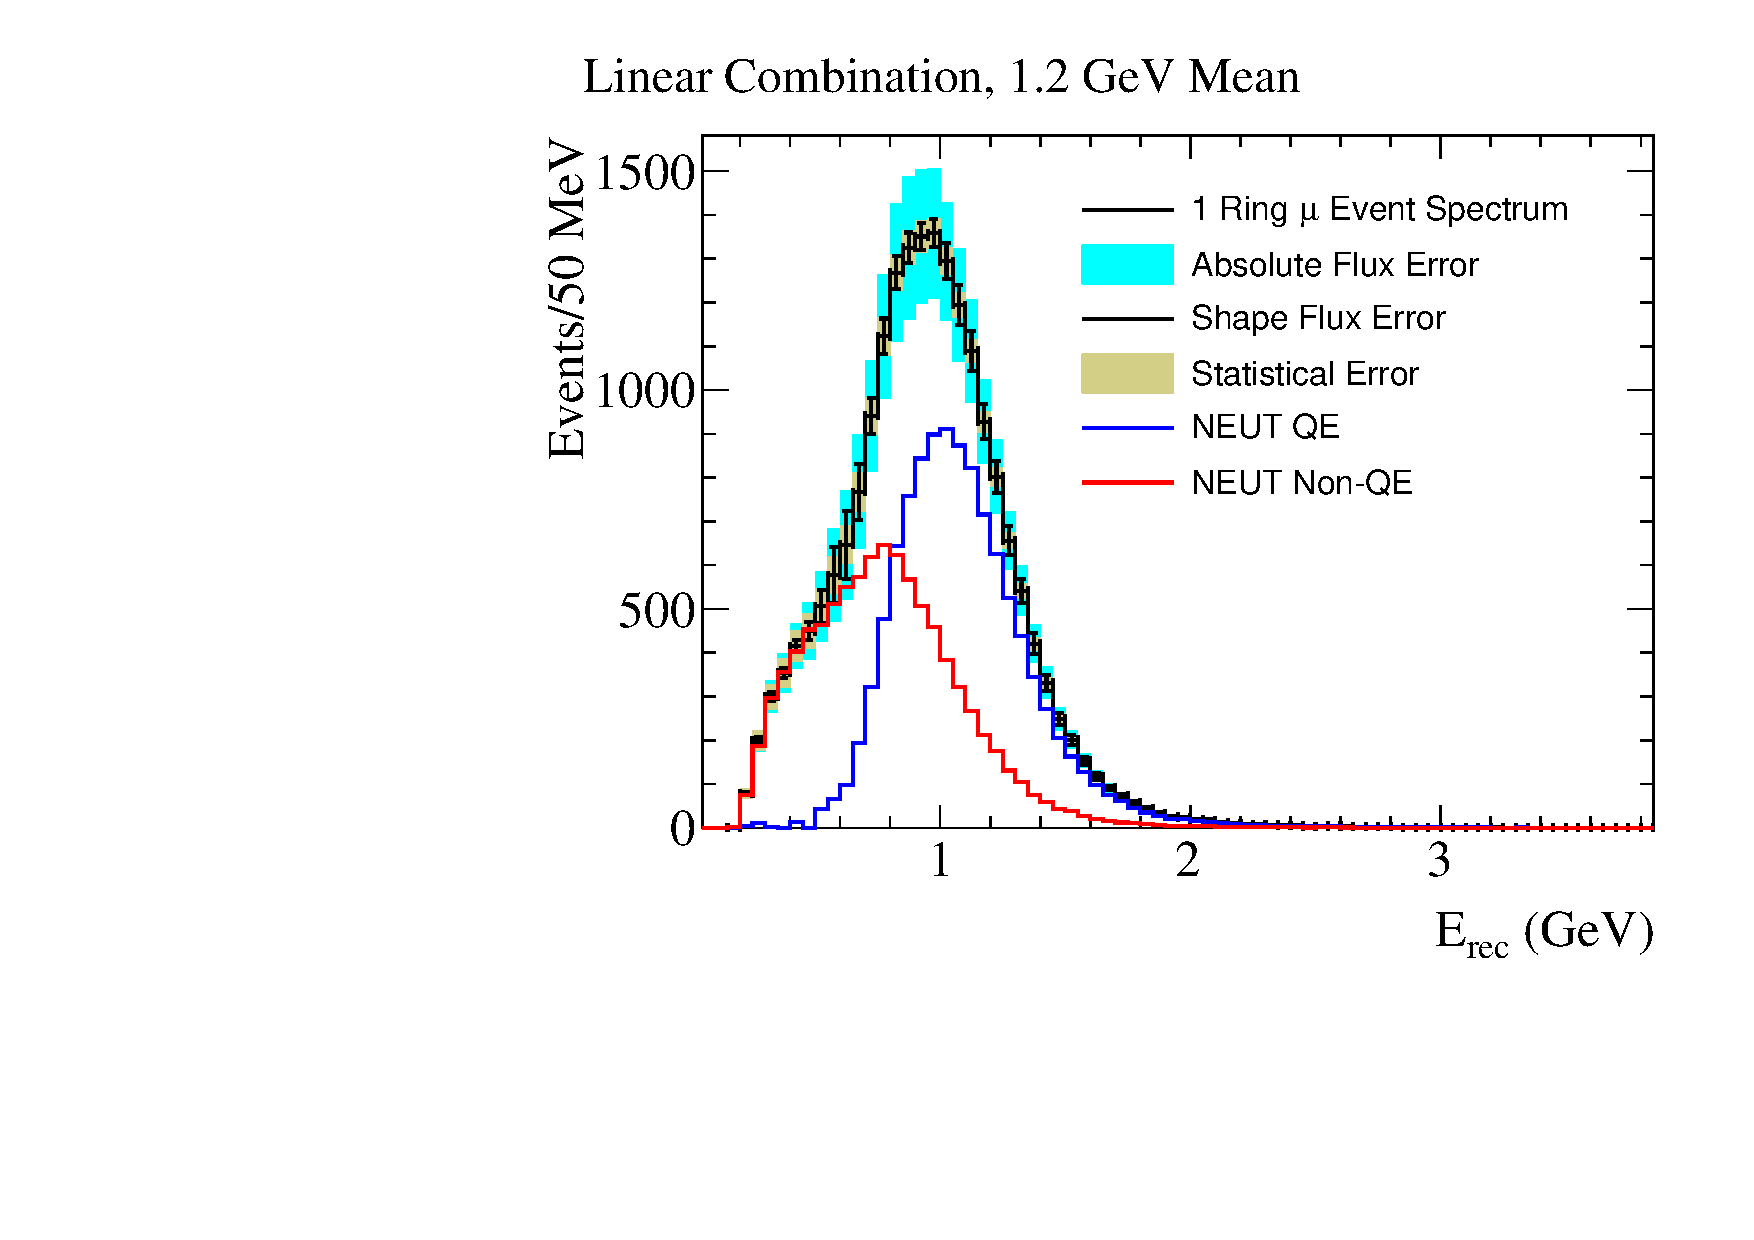
\includegraphics[width=0.45\textwidth]{figures/lc_erec_1200mev.pdf} 
\caption{The reconstructed energy distributions for 1-ring muon candidate events produced using 
``pseudo-monochromatic" spectra centered at 0.6 (top), 0.9 (middle) and 1.2 (bottom) GeV.  The aqua error bars show
the 1 $\sigma$ uncertainty for flux systematic variations, while the black error bars show the flux systematic variation after the
overall normalization uncertainty is removed.  The tan error bars show the statistical uncertainty for samples corresponding to 
 $4.5\times10^{20}$ protons on target.  The red and blue histograms show the contributions from non-quasi-elastic and quasi-elastic
scatters respectively. }
\label{fig:mono_beam_erec}
\end{figure}

The \nuprism technique can be expanded beyond these pseudo-monochromatic beams. This linear combination method can be used to reproduce a wide variety of flux shapes between 0.4 and 1.0 GeV. In particular, as described later in this section, it is possible to reproduce all possible oscillated Super-K spectra with a linear combination of \nuprism measurements, which significantly reduces many of the uncertainties associated with neutrino/nucleus interaction modeling.
